\chapter{Approximation Algorithms}
\section{Introduction}

Many real world optimisation problems are NP-hard so we have little hope of solving them exactly in polynomial time.

Hence we try to approximate the optimal answer instead.

\begin{Def} A factor $c$ approximation algorithm for a minimisation problem is a polytime algorithm that computes for any feasible input instance $I\in \mathcal{I}$ a feasible solution of cost

\[\text{Alg}(I) \leq c \text{OPT}(I)\]

where OPT$(i)$ is the cost of an optimal solution.

Maximisation problems analogous.
\end{Def}

Since we usually don't know the optimal solution we need to find suitable bounds to prove the approximation guarantees of our algorithms. Naturally we will look at bounds derived from Linear Programming approaches.

\section{Metric TSP}

The problem is as with normal TSP but in the case of metric TSP the edge weights obey the triangle inequality.

A classic approximation algorithm is by Christofides. It works similar to the well known spanning tree approximation. 

We first compute a minimum spanning tree. The weight of the MST is a lower bound on any tour, since we get a tree from a tour by removing one edge. We want to build a tour out of the MST without losing too much.

The easy approximation just doubles all the edges, traverses the tree and takes shortcuts (which are actually shorter because of the triangle inequality) to build a tour. This gives a 2-approximation.

The Christofides algorithm improves on this by using the observation that we just need to get rid of the nodes of odd degree in the tree. There has to be an even number of those nodes so we can just connect them using a minimum cost perfect matching (computable in polynomial time, e.g. \href{https://secure.wikimedia.org/wikipedia/en/wiki/Edmonds\%27s\_matching\_algorithm}{Edmond's algorithm} or by Linear Programming). Then the graph becomes eulerian and we can construct a tour out of it.

This is a 1.5 approximation to the optimal cost. Since the MST is a lower bound on OPT we just need to argue that the matching is at most half the weight of the optimal tour.

Let $i_1,\ldots i_{2m}$ be the nodes with odd degree in the same order as in the optimal tour. Consider the two perfect matchings

\[M_1 = \{\{i_1,i_2\},\{i_3,i_4\},\ldots, \{i_{2m-1},i_{2m}\}\} \quad M_2=\{\{i_2,i_3\},\{i_4,i_3\}, \ldots, \{i_{2m},i_1\}\}\]

The optimal tour is the union of both edge sets, so at least one of them has at most weight $1/2$ OPT. Since the eulerian tour on our subgraph has weight $w(\text{MST})+w(\text{matching})$, our claim of a 1.5-approximation is proven.

This is a tight analysis. Consider the graph in figure \ref{Fig:christofidesTight}

\begin{figure}[hbt]
\begin{center}
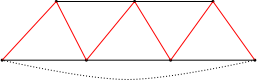
\includegraphics{./images/christofides}
\end{center}
\caption{A tight example for Christofides. MST in red, matching dotted. Edges have unit weight.}
\label{Fig:christofidesTight}
\end{figure}

For general TSP, without the triangle inequality, there is probably no $\alpha(n)$-approximation algorithm for any polynomial time computable function $\alpha$. That is, unless $P=NP$.

If we had such an approximation we could solve the hamiltonian circuit problem which is known to be NP-hard. In the hamiltonian circuit problem we don't have a complete graph like with TSP. We modify by setting all weights in $E$ to $1$ and add edges with weight $\alpha(n)\cdot n$ to obtain a complete graph.

Our assumed $\alpha(n)$ approximation would then solve the problem of finding the circuit. If a circuit exists there is a tour of cost $n$. If no circuit exists the cost of any tour is at least $\alpha(n)n$, because we need to take at least one of the expensive edges. An $\alpha(n)$ approximation can distinguish between these cases, so it can decide whether there is a circuit.

This type of reduction is called gap reduction.

\section{Knapsack}

The Knapsack problems asks to maximise the profit of a subset of items such that the weight of the set doesn't exceed some bound.

A classic approximation is to order the items by "profit density"

\[\frac{c_i}{w_i} \leq \frac{c_j}{w_j} \quad \forall i<j\]

We then take the best of

\[l = \max \{j\in \{1,\ldots, n\}| \sum w_j \leq K\} \qquad \{l+1\}\]

This is a 2-approximation. We can prove this by looking at the LP relaxation of the following ILP

\begin{align*}
\max \quad & \trans c s\\
s.t.\quad & \trans w s \leq K
	& s_i \in \{0,1\} && \forall i
\end{align*}

Obviously OPT$\geq z^*$ where $z^*$ is the optimal value of the relaxation. Since we also have

\[z^* \leq \sum_{j=1}^{k+1} c_j\]

Then we have

\[\max \{\sum_{j=1}^k c_j, c_{k+1}\} \geq \frac 12 \sum_{j=1}^{k+1} c_j \geq \frac 12 z^* \geq \frac 12 OPT\]